\documentclass[10pt,twocolumn,letterpaper]{article}

% Pacotes basicos - maxima compatibilidade Windows
\usepackage{geometry}
\usepackage{times}
\usepackage{titlesec}
\usepackage{url}
\usepackage{graphicx,xcolor,comment,enumerate,multirow,multicol} 
\usepackage{amsmath,amsthm,amsfonts,amssymb,dsfont,mathtools}

% Configuracao da pagina
\geometry{
    letterpaper,
    left=0.75in,
    right=0.75in,
    top=0.75in,
    bottom=1in
}

% Configuracao das secoes
\titleformat{\section}[block]
{\normalfont\fontsize{10}{12}\bfseries}
{\thesection.}{0.5em}{}

% Remove numeracao das paginas
\pagestyle{empty}

% Configuracoes de espacamento
\setlength{\columnsep}{0.25in}
\setlength{\parindent}{0pt}
\setlength{\parskip}{6pt}

\begin{document}

% Titulo centralizado em coluna unica
\twocolumn[
\begin{center}
    {\fontsize{16}{19}\selectfont\bfseries 
    Experimento 1\\ Estudo dirigido sobre estruturas cristalinas}

    \vspace{12pt}
    
    {\fontsize{11}{13}\selectfont 
     Larissa Simões – 232028230, Carlos Eduardo da S. Papa – 232013390, Thiago Ferreira – 232028230}

    \vspace{6pt}   

    {\fontsize{11}{13}\selectfont 
    Turma 01}
    
    \vspace{18pt}
\end{center}
]

\section{OBJETIVOS}

\hspace{1cm} O experimento tem como objetivos identificar a célula unitária e primitiva de uma estrutura cristalina fornecida, determinar planos e direções cristalográficas específicas e calcular suas respectivas densidades planar e linear. Além disso, busca-se relacionar a estrutura cristalina com as propriedades físicas do material e utilizar o software CARINE para visualização, análise e confirmação prática desses conceitos. 

\vspace{.75cm}

\section{INTRODUCAO}
\hspace{1cm} O experimento foi conduzido em duas etapas complementares: uma prática, realizada em laboratório com o auxílio de modelos físicos, e outra computacional, utilizando o software CARINE para simulação e análise detalhada. 

\hspace{1cm} Na etapa prática, o grupo manipulou modelos tridimensionais de estruturas cristalinas, como as redes cúbicas de face centrada (CFC) ou corpo centrado (CCC), para identificar visualmente e geometricamente a célula unitária e primitiva. Foi explicado como identificar e  selecionar os planos cristalográficos específicos e as direções e as atômicas, e então, escolhendo três planos diferentes iniciou-se o experimento com o cálculo das densidades planar e linear para cada caso. Essa abordagem permitiu verificar a anisotropia das propriedades, como variações na densidade atômica em diferentes orientações.

\vspace{.75cm}

\section{MATERIAIS UTILIZADOS}
\begin{itemize}
    \item Modelo da célula unitária hexagonal simples;
    \item Software CARINE Crystallography 3.0. 
\end{itemize}

\vspace{.75cm}

\section{PROCEDIMENTOS EXPERIMENTAIS}

\hspace{1cm} Na primeira parte do experimento, utilizando o modelo cristalino disponibilizado no laboratório, estabeleceu-se inicialmente um sistema de coordenadas que serviu de referência para a análise estrutural. A partir desse sistema, foi possível identificar tanto a célula primitiva quanto a célula unitária da estrutura estudada, ressaltando a diferença entre ambas: enquanto a célula primitiva contém apenas um ponto de rede, representando a menor porção do cristal capaz de reproduzir toda a rede por translação, a célula unitária corresponde a uma forma mais conveniente de representação, que muitas vezes facilita a visualização da simetria do cristal. Assim, com a célula escolhida, demos procedimento à definição dos três planos distintos para estudo, os quais são identificados por meio de seus índices de Miller. Para cada plano determinado, calculou-se a densidade atômica planar, isto é, a quantidade de átomos existentes por unidade de área, e verificou-se quais átomos são interceptados por esse plano. É importante que os três planos definidos possuam densidades planares diferentes, de modo a permitir a comparação entre distintas orientações cristalográficas.

\hspace{1cm} Na segunda parte do experimento, desenvolvida com o auxílio do software CARINE Crystallography 3.0, o procedimento foi similar, mas agora aplicado a um modelo tridimensional gerado virtualmente. Primeiro a partir da célula gerada no software, são definidos novamente três planos distintos, para os quais se calculam as densidades planares e se identificam os átomos que pertencem a cada plano, bem como duas direções cristalográficas diferentes, nas quais são determinadas as densidades lineares correspondentes. Por fim, realizou-se uma pesquisa para identificar qual elemento ou composto cristaliza na mesma forma estrutural do modelo analisado e quais propriedades físicas, elétricas, mecânicas ou químicas estão relacionadas à disposição espacial dos átomos nessa rede.

\vspace{.75cm}

\section{RESULTADOS EXPERIMENTAIS}
\hspace{1cm} Uma vez que a estrutura cristalina utilizada para o estudo foi a célula unitária hexagonal simples, a célula  primitiva relacionada à tal estrutura é um losango tridimensional, ou estrutura trigonal.

\begin{figure}
    \centering
    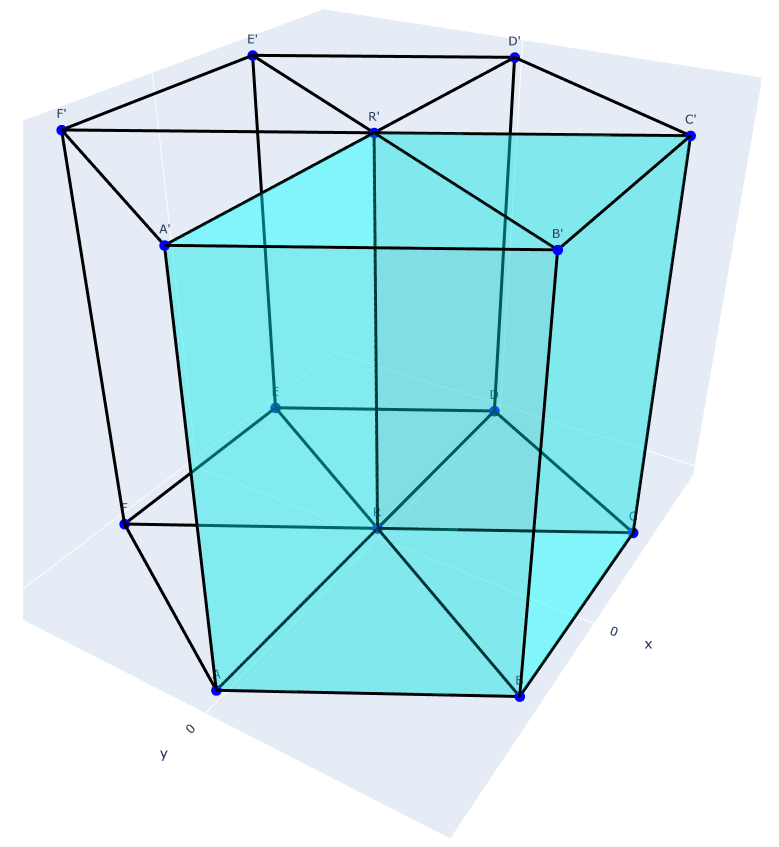
\includegraphics[width=5cm]{PrimitiveCell.png}
    \caption{Célula primitiva da célula hexagonal simples (HS)}
    \label{fig:label}
\end{figure}

\vspace{1cm}

\hspace{1cm} Para a definição dos planos que serão estudados é necessário definir em que pontos o plano desejado intercepta o sistema (x, y, z) escolhido. Escolhemos como referência o sistema no qual o eixo x forma um ângulo de 120º com o eixo y, e os eixos x e y formam 90º com o eixo z.

\vspace{-0.25cm}

\begin{equation*}
    1\;\bar{a} + 1\;\bar{b} + 2\;\bar{c}
\end{equation*}

\vspace{-0.25cm}

\begin{figure}[h]
    \centering
    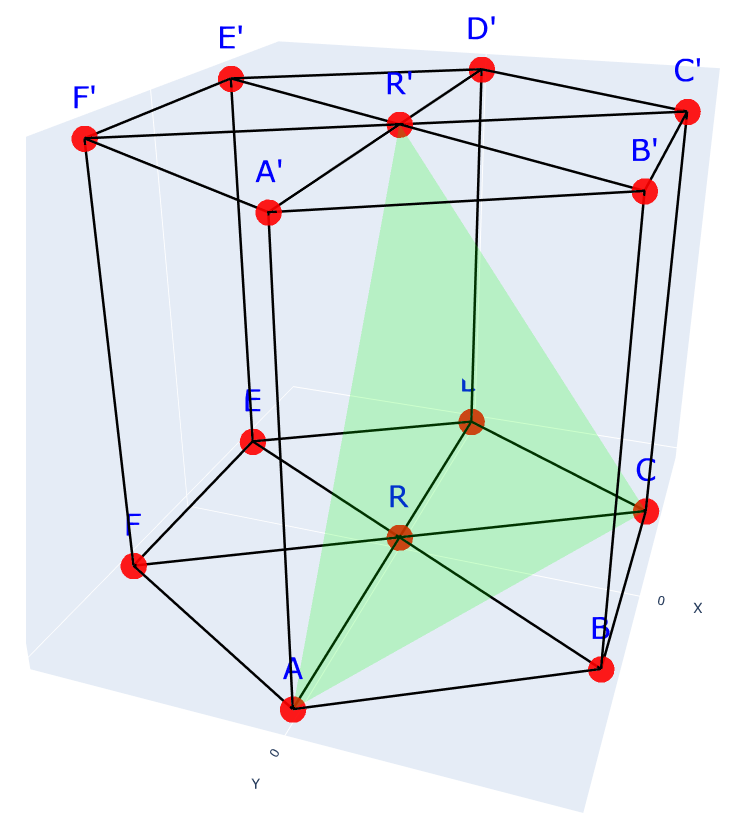
\includegraphics[width=5cm]{Plano1.png}
    \caption{Plano 1}
    \label{fig:label}
\end{figure}

\hspace{1cm} Para retirar a notação de infinito (pelo fato do plano não cortar o eixo) são utilizados os inversos de cada termo.

\vspace{-0.15cm}

\begin{equation*}
    \frac{1}{1}, \frac{1}{1}, \frac{1}{2}
\end{equation*}

\hspace{1cm} Após esse passo devem-se reduzir os valores encontrados aos menores valores inteiros, resultando em:

\vspace{-0.25cm}

\begin{equation*}
    (2 \quad 2 \quad 1)
\end{equation*}

\hspace{1cm} Os inteiros encontrados são chamados de índices de Miller e definem um conjunto de planos paralelos na rede. O índices [2 2 1] representam o plano da figura abaixo. 

\begin{figure}[h]
    \centering
    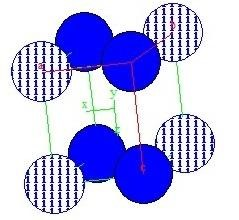
\includegraphics[width=5cm]{fig3.jpg}
    \caption{Plano [2 2 1]}
    \label{fig:label}
\end{figure}

\hspace{1cm} Para que seja definida a densidade planar conta-se o número de átomos que estão contidos no plano e divide-se pela a área do mesmo. Tomando o comprimento do raio da estrutura um valor a temos que a densidade planar para o plana [2 2 1] é dada por:

\begin{equation*}
    \frac{1}{2}\;\bar{a} + \frac{1}{2}\;\bar{b} + 2\;\bar{c}
\end{equation*}

% \vspace{-0.25cm}

% \begin{figure}[h]
%     \centering
%     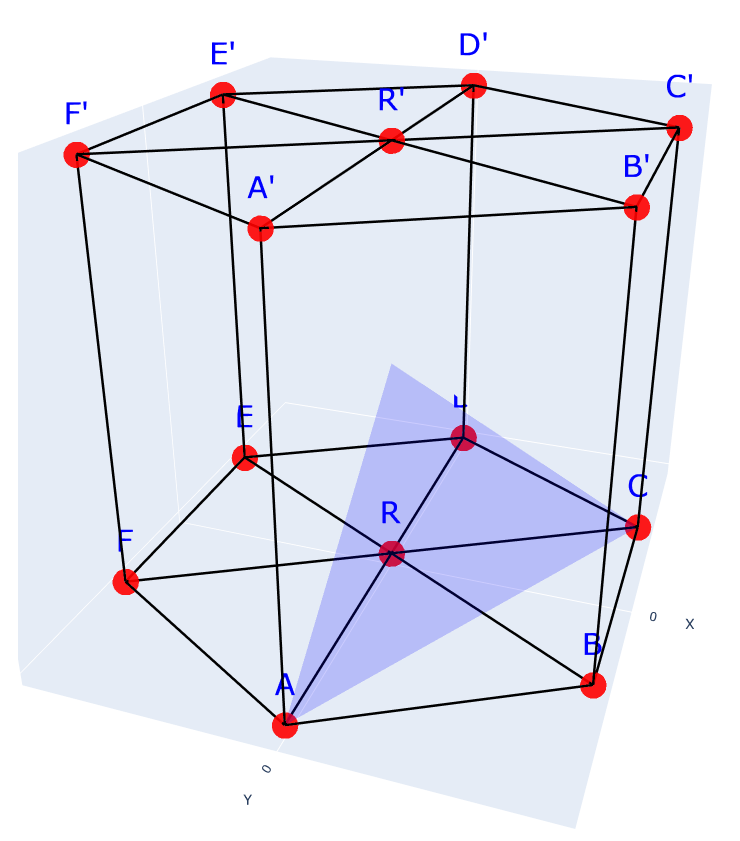
\includegraphics[width=5cm]{Plano2.png}
%     \caption{Plano 2}
%     \label{fig:label}
% \end{figure}

\vspace{-0.25cm}

\begin{equation*}
    2 \;\; , \;\; 2 \;\; , \;\; \frac{1}{2}
\end{equation*}

\hspace{1cm} Reduzindo aos menores valores inteiros encontra-se o seguinte plano:

\vspace{-0.75cm}

\begin{align*}
    [ \; 4 \; 4 \; 1 \;]
\end{align*}

\vspace{-0.5cm}

\begin{figure}[h]
    \centering
    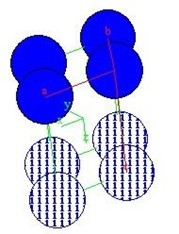
\includegraphics[width=5cm]{fig5.jpg}
    \caption{Plano [4 4 1]}
    \label{fig:label}
\end{figure}

\hspace{1cm} A densidade planar é dada por:

\begin{equation*}
    DP = \frac{1/12}{(\sqrt{3}\;a^2)/2} = \frac{\sqrt{3}}{18\;a^2}
\end{equation*}

\hspace{1cm} Definindo o terceiro plano com o mesmo método utilizado anteriormente temos:

\begin{equation*}
    \frac{1}{1}\;\bar{a} + \frac{1}{1}\;\bar{b} + \frac{1}{2}\;\bar{c}
\end{equation*}

\begin{equation*}
    2 \;\; , \;\; 2 \;\; , \;\; 2
\end{equation*}

\hspace{1cm} Reduzindo, como nos casos anteriores, aos menores valores inteiros é obtido o seguinte plano:

\vspace{-0.5cm}

\begin{align*}
    [ \; 1 \; 1 \; 1 \;]
\end{align*}

\vspace{-0.5cm}

\begin{figure}[h]
    \centering
    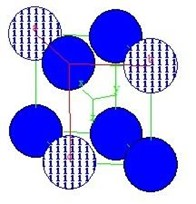
\includegraphics[width=5cm]{fig7.jpg}
    \caption{Plano [1 1 1]}
    \label{fig:label}
\end{figure}

\vspace{-0.25cm}

\begin{equation*}
    DP = \frac{1/4}{(\sqrt{3}\;a^2)} = \frac{\sqrt{3}}{12 \; a^2}
\end{equation*}

\hspace{1cm} Os outros dois planos solicitados foram obtidos da mesma forma, seguindo as etapas mostradas para o plano [2 2 1] marcados entre colchetes. Os resultados foram:

\hspace{1cm} A densidade planar para esse plano é zero, pois o plano não corta nenhum átomo, portanto:

\begin{equation*}
    DP = 0
\end{equation*}

Escolhendo a direção x do sistema (x, y, z) adotado, calculou-se a densidade linear, que é obtida dividindo-se o número de átomos pelo comprimento. A densidade da direção x é então:

\begin{equation*}
    DL = \frac{2\;R}{a} = \frac{\text{diâmetro}}{a} = \frac{\text{1 átomo}}{a}
\end{equation*}

\hspace{1cm} Onde R é o raio do átomo e a é o comprimento do raio da estrutura. Da mesma forma calculou-se a densidade linear da direção z e obteve-se:

\begin{equation*}
    DL = \frac{2\;R}{2\;a} = \frac{\text{diâmetro}}{2\;a} = \frac{\text{1 átomo}}{2\;a}
\end{equation*}

% \vspace{2cm}

\section{ANALISE DOS RESULTADOS EXPERIMENTAIS}

\hspace{1cm} Por meio de uma pesquisa, foi possível  encontrar diversos elementos e compostos cristalizam na forma da rede hexagonal simples, também conhecida como sistema cristalino hexagonal. Entre eles, destacam-se o selênio $(Se)$ e o telúrio $(Te)$, ambos exibindo estruturas hexagonais sob condições específicas. O selênio metálico (forma cinza) cristaliza-se no sistema hexagonal, com parâmetros cristalográficos aproximadamente iguais a $(a) = 436.6 pm$ e $(c) = 495.9 pm$, na estrutura espacial $P3_121$. Esse arranjo é característico de sua forma mais estável e metálica, e confere ao selênio propriedades semicondutoras valiosas em aplicações fotodetectores, fotocopiadoras e células sola Já ores. telúrio, por sua vez, também cristaliza em uma estrutura hexagonal (frequentemente descrita como trigonal, mas com base hexagonal), com constantes de rede aproximadamente $(a) = 0.445 nm$ e $(c) = 0.593 nm$.

\hspace{1cm} Sua estrutura se organiza em cadeias helicoidais ao longo do eixo $(c)$, com átomos de telúrio ligados em espiral; essa morfologia dá origem a formas enantiomórficas, resultando em atividade óptica associada à quiralidade cristalográfica, [Instituto de Metais R]. O telúrio é um semicondutor sensível à luz, exibindo condutividade que varia com a orientação atômica. Essa anisotropia se reflete em propriedades térmicas e elétricas distintas ao longo e perpendicular ao eixo (c), com condutividade térmica variando entre cerca de $3.3 W/m\cdot K$ e $2.1 W/m\cdot K$, e resistividade elétrica também anisotrópica. 

\hspace{1cm} Outro material que cristaliza de forma hexagonal é o grafite, frequentemente descrito como grafite alfa (forma hexagonal mais comum). Cada camada de grafeno do grafite consiste em átomos de carbono ligados em $sp^2$ em um padrão hexagonal bidimensional, com ligações covalentes robustas entre três vizinhos e um elétron $\pi$ deslocalizado que confere excelente condutividade elétrica no plano. As camadas são mantidas unidas por forças de van der Waals fracas, resultando em uma distância intercamadas entre $0.335$ nm e $0.340$ nm, que facilita o deslizamento entre camadas e confere ao grafite sua notável capacidade lubrificante. Além da forma hexagonal, o grafite pode apresentar estrutura romboédrica (grafite $\beta$), com empilhamento ABCABC em vez do ABAB mais comum; essas formas têm propriedades físicas muito semelhantes, mas diferem ligeiramente em empilhamento atômico e comportamento mecânico.

% \vspace{2cm}

\section{CONCLUSAO}

\hspace{1cm} Nesse experimento conseguiu-se alcançar todos os objetivos propostos. Foi possível verificar a concordância dos resultados obtidos com os resultados teóricos estudados.

\hspace{1cm} Apesar de apresentar efeitos satisfatórios, o software Carine trouxe algumas dificuldades, como, por exemplo, não possuir a célula unitária hexagonal simples, o que nos fez trabalhar com a célula primitiva correspondente. Porém, conclui-se a partir do estudo que a célula unitária e formada pela união de 3 células primitivas. E como a celular primitiva é um representativo de toda a rede, podemos encontrar resultados semelhantes para a célula unitária.

\hspace{1cm} Pode-se observar também que a densidade linear varia de acordo com a direção desejada, bem como a densidade planar varia de acordo com o plano adotado.

\hspace{1cm}Observou-se através da avaliação da estrutura cristalina do prisma hexagonal que a geometria do sólido e a disposição espacial dos átomos ajudam a definir as propriedades dos compostos e elementos definidos por tal geometria. 

\section{REFERENCIAS BIBLIOGRAFICAS}

\small
\begin{enumerate}
    \item CESCHIN, Artemis M. Apostila de materiais eletricos e magneticos.
    
    \item \url{https://mateck.com/en/content/119-selen-34se78} "Selenium (Se) - Mateck"
    
    \item \url{https://www.periodic-table.org/Selenium-crystal-structure/} "Selenium - Crystal Structure"
    
    \item \url{https://www.isoflex.com/selenium-se} "ISOFLEX USA - Selenium"
    
    \item \url{https://www.espimetals.com/index.php/technical-data/253-Tellurium.com} "Tellurium - ESPI Metals"
    
    \item \url{https://www.chemicalbook.com/article/tellurium-crystal.htm} "Tellurium Crystal Chemicalbook"
    
    \item \url{https://www.osti.gov/etdeweb/biblio/275148} "The crystal structure and optical activity of tellurium"
    
    \item \url{https://en.institut-seltene-erden.de/seltene-erden-und-metalle/strategische-metalle-2/tellur/} "Tellurium Price, Occurrence, Extraction and Use"
    
    \item \url{https://www.periodic-table.org/tellurium-crystal-structure/} "Tellurium - Crystal Structure"
    
    \item \url{https://en.wikipedia.org/wiki/Tellurium} "Tellurium"
    
    \item \url{https://www.geeksforgeeks.org/chemistry/graphite/} "Graphite - GeeksforGeeks"
    
    \item \url{https://www.infogalactic.com/info/Graphite} "Graphite - Infogalactic"
    
    \item \url{https://unacademy.com/content/jee/study-material/chemistry/structure-of-carbon-allotrope/} "Structure of Carbon Allotrope"
\end{enumerate}

\end{document}